\chapter{Background \& Medicinal Dataset}
\label{chpt:background}
%\setcounter{page}{1}
\nomenclature[1]{HSE}{Health Service Executive} 
\nomenclature[1]{HIS}{Health Information System} 
\nomenclature[1]{Caredoc}{Carlow Emergency Doctors on Call}
\nomenclature[1]{NLP}{Natural Language Processing}
\nomenclature[1]{ED}{Emergency Departments}
\nomenclature[1]{FC}{Frequent Caller}

\nomenclature[1]{ICD}{International Classification of Diseases}
\nomenclature[1]{FTN}{Free-text notes}
\nomenclature[1]{HIPE}{Hospital In-Patient Enquiry}
\nomenclature[1]{SNOMED}{Systematized Nomenclature of Medicine}
\nomenclature[1]{SCOWL}{Spell Checker Oriented Word Lists}
\nomenclature[1]{UMLS}{Unified Medical Language System}
\nomenclature[1]{GMS}{General Medical Services} 
\nomenclature[1]{NER}{Named Entity Recognition} 
\nomenclature[1]{AUC}{Area Under Curve} 
\nomenclature[1]{ROC}{Receiver Operating Characteristic} 
\nomenclature[1]{CDSS}{Clinical Decision Support Systems} 
\nomenclature[1]{NHS}{National Health Service} 

\section{Introduction}


This section describes the relevant background for the research described in this thesis in three separate parts: (i) Out-Of-Hours Healthcare, (ii) Electronic Health Records, and (iii) Frequent Users of primary health care. This background helps motivate the thesis problem, inform the reader about what resources are available in the course of the thesis' investigation, and establish some of the limitations within which the research has to work. 


\section{Out-Of-Hours Health-Care}
\label{Out-Of-Hours_Health-Care}

%Out-of-hours health care provision (OOHC\index{Out-of-hours Health Care}) act as an ad-hoc delivery of triage and treatment, where interactions occur without recourse to a full medical history of the patient in question. Medical histories, relating to patients contacting an OOHC\index{Out-of-hours Health Care}, may reside in several distinct Electronic Health Record (EHR\index{Electronic Health Record}) systems in multiple hospitals or surgeries, which are unavailable to the OOHC\index{Out-of-hours Health Care} in question. As such, although a local solution is optimal for this problem, it follows that the data under investigation is incomplete, heterogeneous, and comprised mostly of noisy textual notes compiled during routine OOHC\index{Out-of-hours Health Care} activities. 

``Out of Hours'' refers to periods of the week where GPs (or family physicians) would be unavailable. \hl{At least in the Irish context under consideration}, these typically relate to periods outside of the standard working day (for instance  periods between 18.00 and 08.00 during weekdays, and the entirely of weekends and public holidays). People telephoning their GP surgeries may be automatically redirected to call operators working on behalf of an OOHC\index{Out-of-hours Health Care} cooperative, depending on what part of the country they are living in. 

OOHC\index{Out-of-hours Health Care} cooperatives are a relatively modern health care delivery system, forming a hybridisation of traditional primary care and telemedicine.  Similar to the structure adopted by the United Kingdom's National Health Service (NHS), % https://www.independent.ie/irish-news/caredoc-irelands-flying-doctors-26133491.html
out-of-hours care in Ireland features a plethora of services, including walk-in centres, out-of-hours centres, telephone consultation, and the emergency department (A\&E) \cite{coombes2016fix}. The complicated pathway that data can take with respect to the organisation under consideration can be seen in Figure \ref{fig:dia0}. 

\begin{figure}[h]
   \centering
   \begin{tabular}{@{}c@{\hspace{.5cm}}c@{}}
 \includegraphics[page=7,width=1.0\textwidth]{Figs/data-flow2.pdf} & 
   \end{tabular}
 \caption{Data flow, agency interaction, and different system usage in relation to OOHC\index{Out-of-hours Health Care} under consideration.}
 \label{fig:dia0}
\end{figure}


The Health Services Executive (HSE) is responsible for the provision of all of Ireland's public health services, both in hospitals and communities across the country. Carlow Emergency Doctors on Call (Caredoc) is a non-profit health care provider, which, through service level arrangements with the HSE, provides OOHC\index{Out-of-hours Health Care} services to patients \cite{cunniffe2016developing}.  The HSE tenders for new services as required, and over the last number of years, Caredoc\index{Caredoc} has been successful in its bids for such contracts \cite{cunniffe2016developing}. 

Figure \ref{fig:dia0} details the flow of both user interaction (in black) and of information (in blue) throughout possible engagement scenarios with Caredoc\index{Caredoc}'s organisation. The scope of Caredoc\index{Caredoc}'s integrated care model is nominally quite broad, but fundamentally it is underpinned by its operation of a call centre which provides the hub for out-of-hours care for quite a wide geographical area. This call centre, dealing directly with patients (labelled \textit{A} in Figure \ref{fig:dia0}) or through a third party calling on the behalf of patients, form the bulk of the information pertaining to patients, held by the organisation. It has been envisioned since its inculcation, that nurse/doctor operated phones, providing both advice and triage, would reduce the burden on other areas of the health service during out-of-hours operation \cite{khistriya2010nhs}.




Caredoc\index{Caredoc} uses a very complicated healthcare software system for the purposes of providing an extensive telemedicine\index{telemedicine} capacity. Nurses operate the phones (\textit{B}) and provide triage, whereupon the caller may be given advice by the nurse, or directed to a doctor who will give advice by phone. Alternatively, the result of the triage may be that a general practitioner locum is sent to conduct a home visit (\textit{C}), or the patient may be asked to visit one of the treatment centres under Caredoc\index{Caredoc}'s management (\textit{D}). Some combination of the above is also possible.  

Regardless of the outcome, the information relating to the call, and any action taking place under Caredoc\index{Caredoc}'s auspices gets recorded in the Electronic Patient Records (\textit{E}), managed by the organisation. If the patient in question was originally redirected from another institution, this information is passed onto these respective organisation. 

\begin{figure}[ht]
   \centering
   \begin{tabular}{@{}c@{\hspace{.2cm}}c@{}}
 \includegraphics[page=3,width=1.0\textwidth]{nightingale.png} & 
   \end{tabular}
 \caption{CDSS\index{Clinical Decision Support Systems} interface used by OOHC\index{Out-of-hours Health Care} phone operators}
 \label{fig:screen2}
\end{figure}



However, the telemedicine\index{telemedicine} and triage described above is not diagnostic in nature. Numerous OOHC\index{Out-of-hours Health Care} take advantage of software for clinical decision making, typically known as clinical decision support systems (CDSS\index{Clinical Decision Support Systems}), and Caredoc\index{Caredoc} is no exception in this regard \cite{kasem2017exploring}. \hl{The software in question, known as Nightingale, is visible in Figure} \ref{fig:screen2}.  CDSS\index{Clinical Decision Support Systems} take in symptoms input by nurses, and make suggestions about the types of conditions the patient may be suffering from. This software is useful is narrowing down the scope of what nurses should consider when dealing with patients, but neither the values input by phone operators, nor the suggested comorbidities derived by the CDSS\index{Clinical Decision Support Systems} are actually recorded.  

The patient records treated in this research may be presented \emph{in media res}, as patients will have had prior interaction with healthcare that is not recorded, and indeed may have possible further  interaction with health infrastructure, that is likewise unavailable within the scope of this project\footnote{as this information is available to neither Caredoc\index{Caredoc}, nor this research}. The data flow within Caredoc\index{Caredoc} is independent of any information relating to patients which may exist in health records in other health care organisations (such as in hospitals, or with the patient's own GP). While Caredoc\index{Caredoc} will transfer data to a patient's GP (or public health nurse, where appropriate) (\textit{F}), the reverse is not true. Consequently, if diagnoses are made in relation to these patients in subsequent analysis, these diagnoses are unlikely to feature within the data possessed by the co-op, unless specifically mentioned by the patient in a potential subsequent interaction between the co-op and the patient. As this information is not available to Caredoc\index{Caredoc}, it thus unavailable to the research described in this thesis.

Consequently, data relating to patients often form little more than snapshots. The incomplete nature of patient medical histories is a typical feature of OOHC\index{Out-of-hours Health Care} \cite{aldosari2017patients}. A decentralised solution with respect to OOHC\index{Out-of-hours Health Care} patient medical informatics is thus a key motivation of this research. 

The software used to record each of episode of care is Ad Astra\index{Ad Astra}\texttrademark \cite{adastra}. Most of the OOHC\index{Out-of-hours Health Care} in both Ireland and the UK use this particular software (or at least some version of it) \cite{natreview}. The limitations of this software are important in terms of the challenges that were present with respect to the data. This chapter will cover some of the preexisting issues relating to data storage that had to be addressed in the scope of our research. 

%system under investigation did not use primary keys to identify patients, and episodes of care were all recorded in unstructured text.~\cite{adastra} [fixbib]
 
 \section{Electronic Health Records}

Electronic Health Records\index{Electronic Health Record}, Electronic Medical Records, and Personal Health Records relate to the digital storage of patient information. These three terms are not quite synonymous, although depending on context they may be used interchangeably. The distinction between the terms relates to how comprehensive the medical information relating to a patient is, with Electronic Medical Records typically relating to information stored in a single institution, Electronic Health Records typically relating to information shared between institutions, and Personal Health Records typically relating to all recorded information about a patient \cite{heart2017review}. However, as is common in nomenclature relating to health care management, usage is not particularly consistent between different researchers. For our purposes we will consider the data system managed by Caredoc\index{Caredoc} to be an Electronic Health Record, as it contains information shared between different organisations, but provides a very disjointed and incomplete record relating to individual patients.  

The concept of an Electronic Health Records was set out in order to close the gap between institution-specific patient data and a comprehensive, longitudinal collection of the patient's health data \cite{quaglio2016health}. During the early adoption of EHR\index{Electronic Health Record}, recording increasingly tended to reflect institutional priorities. These priorities were largely shaped by the social contexts of medical practice, but institutional priorities could only be achievable if there was standardisation in relation to the methods of recording data within the institution's EHR\index{Electronic Health Record}  \cite{doi:10.1111/nup.12112}\hl{.} The consequence of this use of EHR\index{Electronic Health Record} was a de‐emphasis on the patient's narrative as a source of input into the health record, but instead a shift towards representing the patient as a set of data points or metrics \cite{doi:10.1111/nup.12112}. EHR\index{Electronic Health Record}-like systems and e-prescription are priorities in various EU e-Health Action Plan and in the policies of several Member States ( 27 and 22 EU countries respectively). However, the general political commitment to these e-health fields is at different stages of implementation across countries \cite{stroetmann2011european}. Overall, on average, 77.4\% of GPs across Europe store patient consultations in some form of EHR\index{Electronic Health Record} \cite{de2015basic}.

While the digital recording of patient data has been embraced by many countries due to the potential benefits such a policy poses to cost effectiveness of health care provision, accuracy of treatment for patients, and research \cite{peckham2016electronic}, there are a number of extant problems that are common among EHR\index{Electronic Health Record} implementation. Most EHR\index{Electronic Health Record} systems used in health centres are proprietary systems built with different architectures, business rules, information technologies and models, in addition to incompatible clinical terminology. These facts hinder the interoperability among the Health Information Systems (HIS), making it difficult for health professionals to provide continuity of care \cite{gomes2018marcia}.


One significant regional difference between digital medical records in the United States, and those operated in both Ireland and the United Kingdom, is that patient billing forms a large part of the purpose of data recording in the United States, thereby having an impact on the manner in which data is recorded \cite{alpert2019electronic}. Another distinctive regional attribute is that before recent legislative change \cite{kelleher2015privacy}, there has been no legal basis within Ireland for national identifiers for patients. As pointed out by Leonidas et al., legal and political considerations, as well as diverse local complications have made significant long-term hurdles to national implementations of EHR\index{Electronic Health Record} \cite{fragidis2018implementation}. In particular, bottom-up approaches whereby individual hospitals and institutions decide themselves upon what HIS to use, as is typical in the United States, is likely to make interoperability between different institutions' EHR\index{Electronic Health Record} an ongoing challenge \cite{fragidis2018implementation}. The absence of national identifier for patients in Ireland, coupled with legal restrictions and differences in institutional HIS has precluded consistent sharing of patient data between health care services in Ireland. 





\section{Information Systems \\ and Recording Practices}

Electronic Health Records used in the operation of out-of-hours cooperatives are composed of both structured and free-text\index{free-text} clinical notes. However, knowledge discovery currently has very limited application in Caredoc\index{Caredoc}. Identification of patterns within this data, at either a population or individual level, is limited to shallow treatment and narrow parameterisation (i.e. relatively simple queries) \cite{cunniffe2016developing,adastra}. The software used by Caredoc\index{Caredoc}  has a number of structural flaws, such as a lack of primary key for patients, redundant data fields, noisy input, and significant software bugs, which is partially responsible for the restricted scope with which Caredoc\index{Caredoc} can treat its data. 

\begin{figure}[ht]
   \centering
   \begin{tabular}{@{}c@{\hspace{.2cm}}c@{}}
 \includegraphics[page=3,width=1.0\textwidth]{caredoc2.pdf} & 
   \end{tabular}
 \caption{Graphical User Interface used by staff at OOHC\index{Out-of-hours Health Care}, showing text boxes used to record case data.}
 \label{fig:screen1}
\end{figure}


The EHR\index{Electronic Health Record} employed by Caredoc\index{Caredoc} has both parameterised fields and free-text\index{free-text} boxes \cite{adastra}. For the rest of this thesis, data which has been input into the patient record parameters, visible in Figure \ref{fig:screen1}, will be described as `parameterised data'. Like many HIS, each call handled by Caredoc\index{Caredoc} is treated as a unique encounter (or case) \cite{middleton2016experiences}. However, phone operators are able to automatically fill in the parameterised demographic fields relating to the patient being treated. This is achieved by the phone number that is being used to call Caredoc\index{Caredoc} being on record, or the operator manually searching for the patient by name. Despite the Ad Astra\index{Ad Astra} system nominally being a relational database, neither patient nor case records have primary keys\footnote{ Technically all tables in Caredoc\index{Caredoc}'s databases have what the software considers to be primary keys, but these are all automatically incrementing integers which do not enforce normalisation or referential integrity.}.   

EHR\index{Electronic Health Record} documentation is thus encumbered by a number of challenges. In the current system, each provider writes his or her own encounter-based notes, leading to redundancy, fragmentation, and lack of a single shared clinical narrative. This problem is further aggravated when a patient receives care across organisations whose EHRs\index{Electronic Health Record} are not interoperable \cite{warner2019s}. EHRs\index{Electronic Health Record} generally lack standard templates to document additional inputs in structured data fields, and the EHR\index{Electronic Health Record} system that Caredoc\index{Caredoc} operates is no different in relation to this shortcoming. This limitation makes it difficult for practices to find, extract, and track relevant behavioural health and physical health information to monitor quality and improve the delivery of integrated care \cite{cifuentes2015electronic}.

Patient demographic details, as seen in Figure \ref{fig:screen1}, have a large number of fields, including General Medical Services (GMS) Number (if applicable), home address, and telephone number. Most of these are sensitive data, and subject to restricted access based upon data protection legislation \cite{dataprotection2018}. Parametric information also contains details about the call itself, such as the time of day and date that the call was made. However, virtually all information relating to the case in question is treated in non-sanitised free-text boxes, as seen in Figure \ref{fig:screen0}.

Generally, case free-text\index{free-text} records are written by highly skilled physicians and nurses using specialised terms. As is typical in EHR\index{Electronic Health Record}, case record text is very domain specific, depending on which medical discipline it is written in. Each discipline or domain within medicine uses its own set of terms that can be incomprehensible to other disciplines \cite{dalianis2018characteristics}. Patient records are primarily written for hospital internal use and for mnemonic reasons. Daily running notes might contain more spelling errors or noisiness than discharge letters that are read by a larger audience \cite{ehrentraut2012detection}. 


\begin{figure}[h]
   \centering
   \begin{tabular}{@{}c@{\hspace{.5cm}}c@{}}
 \includegraphics[page=4,width=1.0\textwidth]{caredoc2.pdf} & 
   \end{tabular}
 \caption{Graphical User Interface used by staff at OOHC\index{Out-of-hours Health Care}, showing text boxes used to record case data.}
 \label{fig:screen0}
\end{figure}


\subsubsection{Implications for Data Analysis}

Patient records are written under time pressure; the patient record systems
do not contain any spelling correction (or grammar checking) system due to the
difficulties of building this type of functionality in the context of the complicated, non-standard
vocabulary used within health care \cite{dalianis2018characteristics}. Extracting features from non-annotated, unstructured text produces distinct challenges. Clinical text is designed to be human interpretable by persons with domain specific knowledge who can infer meaning from context. The manner in which information is recorded is not only inconsistent from person to person but rather, is dirty: typically exhibiting spelling mistakes, shorthand, colloquial phrases, and truncated grammar. Although a best practices guide has been developed by the HSE for the way in which acronyms should be recorded \cite{abbreviations}, Caredoc\index{Caredoc} (like many medical organisations) follows no consistent rules for the way in which abbreviations, acronyms, and shorthand should be recorded in free-text\index{free-text} \cite{cunniffe2016developing}. \hl{Free-text notes could be contributed to by call centre staff, by nurses interacting with the patient either on the phone or in person, or by GP locums, again interacting with the patient either on the phone or in person} (Figure \ref{fig:dia0}). No indication is given in the text of the type of staff member who has written the notes in question. As such, a single disease, medication, or symptom can consequently be written using a multitude of variants. The terse writing style and heavy use of contractions consequently makes traditional natural language processing (NLP)\index{Natural Language Processing} solutions largely inappropriate in this setting.







%We identified 3 EHR\index{Electronic Health Record} challenges common among practices integrating care. First, practices hired new types of clinicians, such as psychologists in primary care practices and nurse practitioners in community mental health centres, who generated data not previously documented or tracked by existing EHR\index{Electronic Health Record} systems (e.g., patient health questionnaire  scores, behavioural health visit notes, consultation notes, referrals to outside services). EHRs generally lacked standard templates to document these additional inputs in structured data fields. This limitation made it difficult for practices to find, extract, and track relevant behavioural health and physical health information to monitor quality and improve the delivery of integrated care. Second, integrated teams had specific communication and care coordination needs, such as use of shared care plans to coordinate tasks for patients receiving integrated care services, and reported needing the ability to see when each other's tasks were completed. EHRs typically did not have templates that supported shared care plans for both primary care and behavioural health needs. However, EHRs that had tasking functions were helpful in enabling some types of communication and coordination between team members. Third, EHRs were not interoperable with other EHR\index{Electronic Health Record} systems or with tablet devices used by practices to administer behavioural health screening surveys. This lack of system interoperability created further barriers to document patient encounters, access needed information at the point of care, and easily and consistently communicate information between primary care and BHCs.
%\cite{cifuentes2015electronic}






%Redundant documentation \cite{warner2019s} 



Text mining of medical information can extract features from clinical digital reports. Features from clinical data typically represent medical concepts, such as symptoms, diagnoses and prescriptions. Using this data, partial medical histories can be constructed for individuals. A more detailed examination of what form this sort of feature takes will be given below.

%Extracting features from non-annotated, unstructured text produces distinct challenges. Clinical text is designed to be human interpretable by persons with domain specific knowledge who can infer meaning from context. The manner in which information is recorded is not only inconsistent from person to person but rather, is dirty: typically exhibiting spelling mistakes, shorthand, colloquial phrases, and truncated grammar. Although a best practices guide exists for the way in which acronyms should be recorded,~\cite{abbreviations} it is not closely adhered to, and a single disease can consequently be written using a multitude of variants. The terse writing style and abbreviation of many words consequently makes traditional NLP solutions inappropriate. Furthermore, not only are words of unequal value, some nouns would prove counter-productive if extracted as features due to their contextual negation. 
 
 
 
 Instead of a conventional relational database, cases and patients are not linked, and in place of a foreign patient key being recorded in case information, a small summary of the patient’s details (such as their name, date of birth, registered surgery, etc.) is included in the cases table for each entry. These patient details are both complete and reliable however, due to their being automatically populated from the respective patient’s table by the operator on duty. Cases, meanwhile, use a non-unique index, excluding nulls. 



Cases have two different types of duplicate: the first appears immediately after its mimesis and will typically include appended free-text\index{free-text} information about the entry that preceded it, but may also feature different attribute information, depending on the source of the entry. The second type of duplicate merely shares the same key as some other case, but will have no other direct connection to these cases. 

In accordance with the Data Protection Act (2003), potentially identifying features relating to patients cannot be included in data available to access by a third party \cite{commissioner2004data}. This had a significant bearing on the manner in which data was to be extracted, if vital semantic information was to be maintained for the purposes of the research during mandatory redaction processes.

It was thus necessary to develop a means to successfully build patient profiles from this data, including the deletion of duplicate information, linking of cases with patients, and tracking of changes in cases over time. 


\section{Frequent Users}
\label{section:frequent-users-rr}
%holmstrom2017frequent
%Frequent attenders have been the subject of researchers’ attention, often from an emergency care or general practitioner (GP) perspective. Patient and nurse perspectives are investigated in a minority of the studies (Malone 1996, Neal et al. 2000, Wiklund‐Gustin 2011, 2013). Furthermore, there is no consensus regarding the definition of a frequent attender. It could be defined as a person with three or more healthcare contacts per year (Buja et al.2015) or a person with 30 consultations or more within a 2‐year period (Patel et al. 2015). In the literature, factors associated with frequent use of healthcare services have been examined (Bergh et al. 2007, Buja et al.2015, Patel et al. 2015). The few studies conducted from a patient perspective have shown that frequent attenders of primary healthcare services describe a situation where they feel mistrusted and rejected by healthcare providers (Neal et al. 2000, Wiklund‐Gustin 2011, 2013). There are challenges in relation to the potential overuse and unnecessary use of services for healthcare organizations with finite resources. Frequent attenders are considered to increase the workload and costs of primary health care (Buja et al. 2015, Patel et al. 2015). Furthermore, there is no self‐evident way of helping frequent attenders, as their dependence on the healthcare sector might in fact be counterproductive (Spittal et al. 2015).

The problem of high recurring patients has long been acknowledged in healthcare. High recurring patients are, however, a complicated subset of subjects that are difficult to classify. Not only do these patients have disparate demographic details, but the symptoms with which they present to primary care staff are diverse, and rarely indicate their belonging to this subgroup. This thesis will give an overview of the extant literature concerning frequent users of healthcare, why the prediction of such patients could be a significant contribution to healthcare delivery, and how general principles relating to frequent users ties into our research. In particular, this thesis will discuss what measures currently exist for predicting such patients, and how our proposed model improves upon these approaches.

While frequent users of healthcare facilities has been a perennial issue, relatively little research has been conducted in relation to frequent use in the context of telemedicine\index{telemedicine}. Most extant health-care management documentation relating to frequent use has focused exclusively upon frequent attendance in secondary healthcare, particularly that of emergency departments (ED) \cite{jelinek2008frequent,hockey2014understanding,khatua2019tale}. Such research has largely been conducted with the motivation of moving these types of patients to primary care (e.g. GPs or ambulatory healthcare centres). There is growing understanding that interventionist measures, while an area of critical importance, should be patient focused, and not merely shift responsibility for care of such patients \cite{hockey2014understanding}. It is accepted that patients who repeatedly use either primary or secondary healthcare have ongoing medical issues which are not being resolved, despite their repeated use of healthcare facilities \cite{morriss2007cluster}. 

Studies that have been conducted in recent years concerning phone based interaction between the public and medical staff have shown strong correlations between Frequent Attenders (FA) and Frequent Callers (FC) of healthcare facilities \cite{krieg2016individual}. There is a consistent pattern whereby frequent users of emergency healthcare have a tendency to be frequent users of primary healthcare \cite{byrne2003frequent,krieg2016individual}. As such, frequent attendance and calling are not isolated issues, but share a common cohort. Notwithstanding the type of healthcare offered, frequent usage is a ubiquitous issue that faces all levels and forms of primary and secondary healthcare offered to the public. This thesis will consequently discuss research relating to  FA in the context of ED, as well as recent research relating to FC, despite the largely telemedical\index{telemedicine} nature of the OOHC\index{Out-of-hours Health Care} under investigation.  

There is no standard definition of what constitutes a high use patient in any sector of healthcare provision. Not only has there been little work carried out with the aspiration of creating a universal means to delineate high users from non-high users, some researchers, such as Billings et al. say that to do so is not even clearly useful from a policy standpoint \cite{billings2013dispelling}. By convention institutions typically have their own specific definition for frequent use. However, there are qualities which are prevalent across the medical domain in relation to these users.

Despite it being self evident that frequent users are characterised by the high frequency with which they interact with healthcare provision, the terminology relating to such patients is nonetheless volatile. The actual threshold for what is considered to be `high' use varies between institutions, and usually depends on the type of healthcare being considered. For instance, the number of attendances deemed to  constitute a FA of secondary healthcare is typically significantly lower than the number of phone calls used to define a FC \cite{edwards2015frequent}. Furthermore, the definition of a frequent user may depend on the manner in which healthcare is offered on a nationwide level, while the specific threshold used to determine how many contacts constitutes “frequent use” fluctuates significantly between different countries, regions, and even particular departments. In countries where public healthcare is free, such as in Denmark, Ireland, and the United Kingdom, any difference in the proportion of frequent attenders must be explained by other factors than economic \cite{pasgaard2018social}. 


A growing tendency within research into frequent users has been to create delineations between frequent and high frequent use of health care facilities, as this can help identify divergent characteristics between different types of frequent usage. For instance a study in 2019 by Bhroin et al. in the A\&E department of Mercy University Hospital in Ireland (in an administrative region adjacent to the area that is covered by the OOHC\index{Out-of-hours Health Care} we are examining) classified high frequent attender as patients with between 13 to 30 Emergency Department visits per year, and very high frequent attenders as those with over 30 Emergency Department visits \cite{bhroin2019profiling}. It is worth noting that this is strikingly higher than what may be typically seen in classification of ED FA in the United States. % \todo{THIS IS HIGHER THAN WOULD BE SEEN IN HOSPITALS IN THE US}. 
 Helplines on the other hand typically use a threshold of one call a week to define FC. No study has shown a threshold number at which striking differences in resources, demographics, or clinical import are observed in relation to a specific threshold for emergency department FA \cite{lacalle2010frequent}.


%\todo{The particular service that is being offered by a given healthcare provider may also inform the nature of frequent users that it is presented with. For instance, while a phone based crisis helpline may experience frequent users who are WHAT WHAT WHAT , emergency helplines for requesting ambulances have found frequent users to typically be WHAT WHAT WHAT . Similarly, WHAT WHAT WHAT.} 



%While all phone based healthcare constitutes primary healthcare, the particular service that is being provided by telephone may also inform the nature of frequent users. *** ARE THERE  DIFFERENT CHARACTERISTICS FOR PATIENTS WHO CALL LIFELINE THAN CALL CAREDOC? ***
%Although the use of phone based crisis helplines for providing reassurance or advice in the context of psychological distress would typically appear to have a less utilitarian profile than emergency helplines for requesting ambulances. Nevertheless research shows that no matter what  While this may make helplines like the Samaratans or Lifeline particularly susceptible to frequent usage, 


While mental and psychological disease, and drug abuse, have long been attributed to FA of ED \cite{malins2016cognitive,byrne2003frequent} recent literature has pointed to a far more complicated set of morbidities and co-morbidities that are present in patients that are classified as frequent users. Frequent users also tend to originate from a wide range of backgrounds. There is significant disagreement between researchers on whether demographic details have any significant predictive power in relation to such patients.  

Healthcare staff have described both the psychological and temporal difficulties that these patients pose on their facilities. Frequent use has been associated with frustration both on the part of the patient and also the healthcare staff \cite{holmstrom2017frequent}.  Historically frequent users have erroneously been considered to be ``time wasters'' \cite{pirkis2016frequent}. This viewpoint nevertheless reflects the difficulties of treating such patients, as they invariably present with underlying issues which are not easily resolvable by the staff that are treating them (indeed these issues may fall under the category of medically unexplained symptoms \cite{baker2013pilot}, that is physical symptoms, which are inadequately explained, or not at all, by somatic disease \cite{creed2011medically}). Additionally they may present with increased  psychological requirements,  and interaction may be complicated by the nominal reason for their contacting the healthcare provider.


Frequent use of helplines, emergency departments, and primary care represent complex unmet needs, which warrant close attention to inform optimal healthcare pathways \cite{daniels2018better,byrne2003frequent,spence2014frequent}.  Emergency and OOHC\index{Out-of-hours Health Care} are designed for emergency and routine primary care (as their names may suggest), and are not designed for the complex needs of frequent users. Ultimately the treatment that is provided to this cohort is both short-term, and superficial, and does not engage with the primary issue concerning these patients. Consequently recent research has started to be developed whereby these patients are not considered to be normal patients behaving in an aberrant (and thus wrong) fashion, but rather a group that require specialised treatment\cite{malins2016cognitive,buja2015determines}. \hl{Furthermore}, strategies need to be developed to attempt to tackle underlying issues which are bringing these types of patients into contact with healthcare provision.  

Intervention specifically designed to target and treat frequent users has shown significant promise, not only in terms of a reduction in the frequency with which such patients present to healthcare operators, but also in terms of the acuity of treatment and satisfaction of patients \cite{billings2013dispelling}. However, the means to develop ways of identifying these patients is non-trivial. If the healthcare facility is using EHR\index{Electronic Health Record} to record data, a frequent user of the same healthcare facility can be identified simply by searching for how many previous encounters the healthcare facility has had with that patient.  This is nonetheless an undesirable approach, as it necessitates that a patient already be established as a frequent user before any sort of interventionist approach can be adopted. Furthermore, the lack of interoperability between the EHR\index{Electronic Health Record} of different institutions is a widespread and ongoing problem \cite{reisman2017ehrs}. Interactions between a patient and a given health care provider is typically isolated from any other interaction that that patient may have had with other health care provision. This is not only true in terms of types of healthcare provision (e.g. GP, OOHC\index{Out-of-hours Health Care}, ED) but even between different institutions providing the same type of treatment. Consequently frequent users are almost exclusively considered in terms of their interactions with a single institution.  

The primary complaint presented to healthcare staff is typically only tangentially related to ongoing reasons for such patients contacting the healthcare provider \cite{bhroin2019profiling}. As a result of this there tends to be obfuscation of the main issues facing these patients, which adds to difficulties of discoverability. Even where literature agrees that certain diseases have high correlation with frequency of presentation, major issues arise in the episodic nature of treatment in OOHC\index{Out-of-hours Health Care} \cite{krieg2016individual}. The specific, or at least nominal reason for the patient appearing in an ED, or contacting an OOHC\index{Out-of-hours Health Care} centre by phone, may be different with each visit.  This can hide underlying conditions. Frequent users are at risk of becoming serial users (having consistent patterns of usage over multiple years). Other frequent users, on the other hand, may be acute (having a large number of contacts over a relatively short period of time).  Attrition rates of those who remain frequent users decrease over time, making them an ideal group for targeted interventions \cite{krieg2016individual}. 

The points of contact with the  OOHC\index{Out-of-hours Health Care} under investigation in this thesis predominantly concern FC, although other areas of primary care are factored into  the collected data (such as visits to treatment centres and GP home visits). GP interaction can be  in-person or through advice given over the phone.  The actual treatment offered is typically decided by nurse triage staff while on the phone to either the patient, or someone calling on behalf of the patient \cite{graversen2019quality}. Patients may also present directly at treatment centres, though this is a significantly less common form of interaction with the OOHC\index{Out-of-hours Health Care} organisation. 


While there were many factors that differentiated non-FAs from FAs in general, persistent frequent attendance was specifically associated with gender, baseline reports of depression, self-reported physical conditions and disability, and medication use \cite{pymont2015longitudinal}.







 
\section{Description of Medicinal Dataset}
\label{chpt:medicial-dataset}

\begin{comment}

\newtheorem{theorem}{Theorem}


\begin{theorem}[Argument Principle]
If $f(z)$ is a meromorphic function inside and on some closed contour $C$, and $f$ has no zeros or poles on $C$, then
\begin{equation}
\label{eq:1}
\oint \frac{f'(z)}{f(z)} dz = 2\pi i(N-P)
\end{equation}
\end{theorem}


%https://tex.stackexchange.com/questions/240243/getting-gif-and-or-moving-images-into-a-latex-presentation/240387#240387




\begin{frame}{Embedded Animation}
%  \animategraphics[loop,controls,width=\linewidth]{10}{skeleton}{0}{16}
\end{frame}


\end{comment}
% USE THE 32 upvoted answer

%\foreach \n in {1,...,8} {
%\begin{tikzpicture}[scale=10,rotate=90]
%\draw (-.1,-.2) rectangle (.4,0.2);
%\draw
%    [blue,opacity=0.5,line width=0.1cm,line cap=round]
%    l-system [l-system={A,axiom=A
%    ,order=\n,angle=45,step=0.25cm}];
%\end{tikzpicture}
%}
%

%THIS IS A SUPERVISED DEEP LEARNING TASK!!! 
Once the detection and prediction of frequent users had been identified as a priority by our partners in Caredoc\index{Caredoc}, a means of extraction, processing, and testing had to be formulated. Moreover we had to develop a classifier with which patient cases could be analysed. Given that the majority of valuable case data resided in unstructured FTN\index{free-text}, our determination was that the manner in which this data was treated would be key to solving this primary research question. First this would necessitate the processing of the Caredoc\index{Caredoc} databases, the most important step being the association of case data with individual patients. Once a star schema of patients was developed, generic cleaning processes would have to be performed on the FTN themselves.


This section will relate the process of creating the corpus upon which all further experimentation in this thesis is based: the methods used in the extraction, anonymisation, and means of ensuring data integrity. Once this is complete, an in-depth description of the resultant dataset will be performed.


%
%---
%Significant amount of meta-data, and some patient-specific data. These features were fairly representative of EHR\index{Electronic Health Record}. 
%---


%COMBINATION OF FTN ATTRIBUTES


\subsection{Data Integration}

A non-volatile (i.e. offline), time-variant store of historical data designed around the subject of patients was a necessary precursor to the research of this thesis. To this end we sought to consolidate Caredoc\index{Caredoc}'s data in a multidimensional space in a repository maintained separately from the organisation’s operational databases. This allowed for the integration of a variety of application systems.  



\begin{figure}[ht]
   \centering
   \begin{tabular}{@{}c@{\hspace{.5cm}}c@{}}
 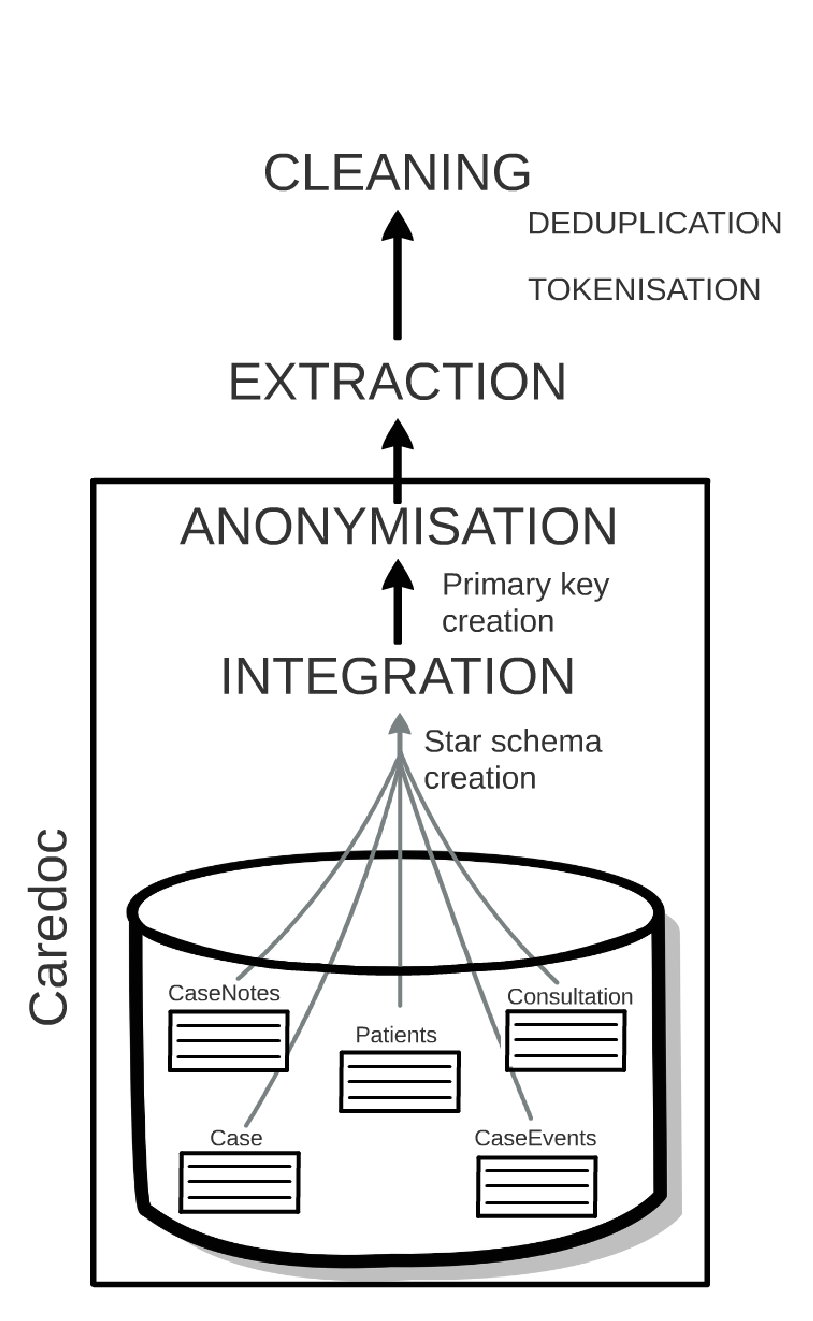
\includegraphics[page=1,width=0.7\textwidth]{data-flow3.pdf} & 
   \end{tabular}
  \caption{\hl{Data selection and extraction processes} used in relation to associate operational systems.}
 \label{fig:data-mining}
\end{figure}


The first step in this process involved collaboration with the domain experts of Caredoc\index{Caredoc} and identification of broad research goals, the latter of which have since formed the basis for this thesis. Once ethical approval for this research had been achieved, a series of goals were developed, as can be seen in Figure \ref{fig:data-mining}, that would be necessary for our use of this data. Removing historical data to a location where it could be subject to analysis without jeopardising systems that are in active use in a live medicinal setting was a research prerequisite. In order to achieve this an iterative set of queries which could extract data from the various sources under Caredoc\index{Caredoc}'s supervision had to be developed. This integration of data, from numerous independent tables, was primarily achieved using the pseudo foreign keys that were in operation in the Caredoc\index{Caredoc} systems.\footnote{An example of the internal Caredoc\index{Caredoc} data systems can be seen in Figure \ref{fig:internal-caredoc} in the appendices. Note that many of the attributes and tables in Caredoc\index{Caredoc}'s systems are not operable for multiple reasons, such as some of the tables being inherited from similar systems from the NHS and not being applicable in an Irish setting.} A single table which would form the corpus for our research was formed from the extracted information from the Caredoc\index{Caredoc} systems using the star schema \cite{han2011data}. As this was being created, a primary key for patients had to be simultaneously generated in order to help bind this data in a normalised manner. This key was produced using SHA-256 hashing \cite{rachmawati2018comparative} over a combination of patient name and date of birth. Patient personal details (such as name, day and month of birth, phone number, and address) were excluded from the process of data integration, ensuring that the corpus that was ultimately extracted from Caredoc\index{Caredoc}'s systems would contain anonymised patient details. 

In Figure \ref{fig:data-mining}, \textit{CaseNotes} is a linking table that contains a unique hexadecimal to reference other tables. \textit{Case} is the main table that contains information relating to a specific case for a patient. \textit{Consultation} is the main table that contains consultation information relating to a case for a specific patient. \textit{CaseEvents} contains information relating to a specific case and the time line for what happened to the case. \textit{Patients} contains the information relating to a patient who may have multiple cases attached to them. The extraction process flattened all of this information into a single table, from which all the research in this thesis is predicated. The rest of this chapter will give a high level analysis of this data, and the significance it may pose to this research.

Because the Caredoc\index{Caredoc} databases were non-normalised, duplicate case data could be created during normal operation of the OOHC\index{Out-of-hours Health Care}, and consequently made up part of the corpus that was extracted from Caredoc\index{Caredoc}. Absolute duplicate cases and empty cases were both straightforward to eliminate from the repository. However, staff at Caredoc\index{Caredoc} when dealing with patients occasionally copied case data and edited this copied data, instead of editing the original case entry. We accordingly developed an algorithm to search for exact strings in cases with identical case numbers, and deleted the original case data that had been copied by the phone operator. This reduced the final corpus from 310549 to 294337 cases.    

  \begin{figure}[ht]
   \centering
   \begin{tabular}{@{}c@{\hspace{.2cm}}c@{}}
 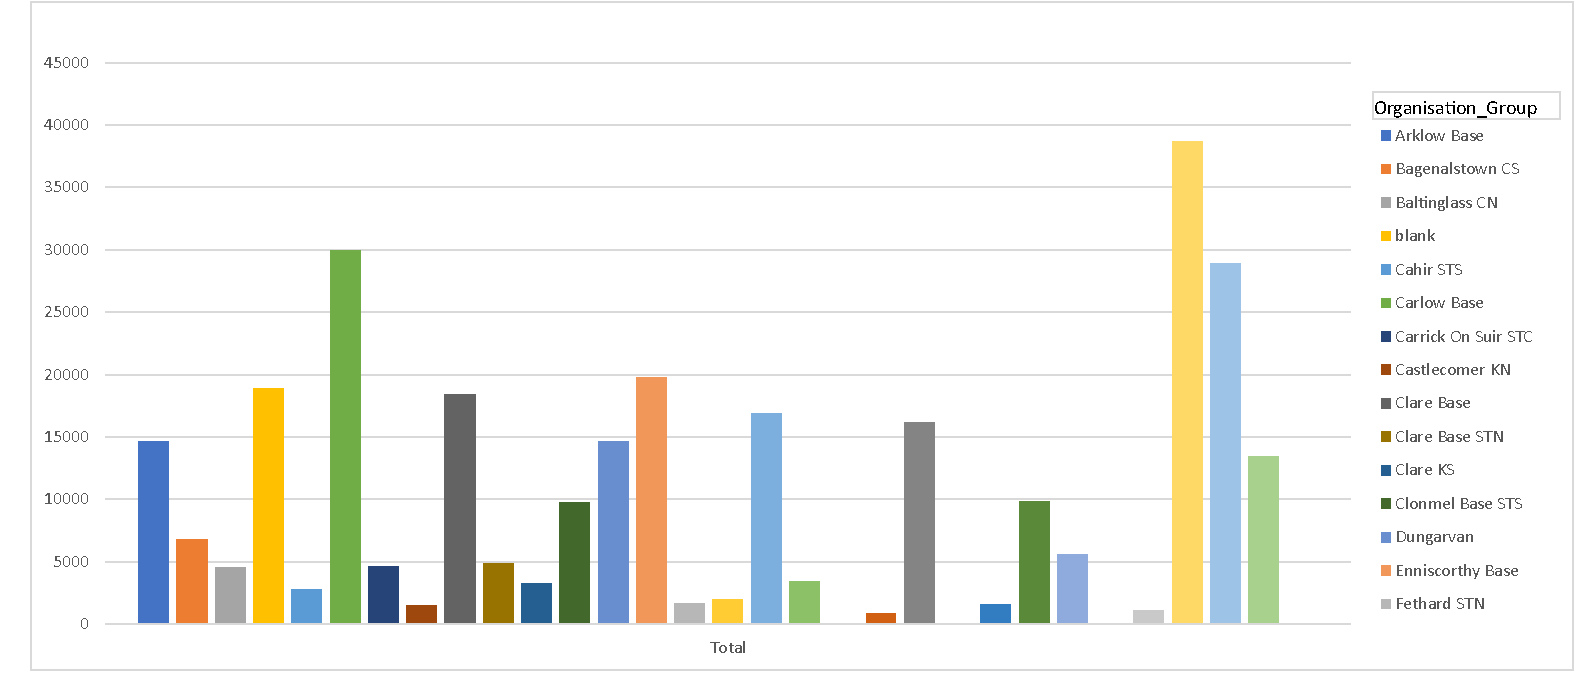
\includegraphics[page=1,width=1.20\textwidth]{graph-origin.pdf} & 
   \end{tabular}
  \caption{The collated dataset contained information obtained from a wide range of sources.}
 \label{fig:info-origins}
\end{figure}



%Extracting features from non-annotated, unstructured text creates distinct challenges. Clinical text is a patois designed to be human interpretable by persons with health care backgrounds who can infer meaning from context. The manner in which information is recorded is not only inconsistent from person to person, but moreover, is dirty: typically exhibiting spelling mistakes, shorthand, colloquial phrases, and truncated grammar. Although best practise guides exist which describe ways in which medical terms should be recorded by healthcare professionals, e.g. \cite{abbreviations}, there is no standard for the industry as a whole and adoption by individuals may be discretionary. Typically, as is the case in the dataset under investigation, medications, signs, and diseases can be written using a multitude of variants. The terse writing style and abbreviation of many words consequently restricts the number of Natural Language Processing (NLP) approaches which would be suitable to use upon the corpus \cite{tsujii2011computational}. Entirely ignoring syntactic context in favour of lexeme specific approaches (e.g. Bag-of-Word variants)\cite{zhang2010understanding} would not necessarily be appropriate. Not only is context important in developing robust means of cleaning the data, but the environment within which lexemes appear may have a substantial bearing on their importance (for instance, contextual negation) \cite{elkin2005controlled}.




%While this factor relating to the data in question is to some degree a technical deficiency owing to the manner in which telemedicine works in this particular environment, even were an exhaustive medical history of the patient available to the call-handler, its practical value would be diminished by the necessity for call-handlers to promptly handle and conclude calls. Manually parsing large volumes of medical information relating to the patient in question would hamper the performance of a triage. From the point of view of any algorithm that is developed within the scope of our research, the potential features available are inherently limited by the incomplete medical histories that are recorded about patients.       

\subsection{Description of dataset}
\label{section:dataset-description}





The aim of this section is to provide an overview of the key attributes of the dataset. Although some of the parametric data looked promising for predictive analysis, the inconsistent use and overly generic nature of these features by call operators told against their overall importance, as shall be explored below.

Very little parametric data was supplied in relation to patients themselves. While this was partially due to the anonymisation processes undertaken during data extraction, the patient parameters which were absent from this research, such as patients' addresses or phone numbers, would have likely provided meagre value from an analysis perspective. Personal medical data like patient height, weight, blood type, etc. were not collected by Caredoc\index{Caredoc} owing to the way in which OOHC\index{Out-of-hours Health Care} platforms function.     
 
% IN DEPTH DESCRIPTION OF DATASET
 
 %WHAT MAKES AN AVERAGE PATIENT
 
 %WHAT MAKES A FREQUENT USER?
 
 %EXPERT SYSTEMS should go into chapter 2.





 \begin{comment}
 \begin{table}[htbp]
 \caption{Description of numerical based information in extracted corpus}
\begin{center}
\begin{tabular}{|l|l|l|l|l|}
\hline
 &  mean & stdv &  min &  max  \\ \hline

dob &  1980.646 &  27.424 &  1900 &  2020  \\ \hline

month &  6.591 &  3.56 &  1.00 &  12  \\ \hline

day &  15.987 &  8.836 &  1.00 &  31 \\ \hline

cases &  6.35 &  23.629 &  1.00 &  395 \\ \hline

weekday &  3.929 &  2.399 &  1.00 &  7  \\ \hline

hour &  15.217 &  5.478 &  1.00 &  23 \\ \hline

minute  & 28.682 &  17.258 &  0.00 &  59 \\ \hline

second &  29.416 &  17.296 &  0.00 &  59 \\ \hline

case-no &  58554.323 &  23856.083 &  10001 &  99999 \\ \hline

Cons\_Time\_Taken  & 8.08 &  8.709  & 0.00 &  356 \\ \hline

\hline  
 \end{tabular}
 \end{center}

\end{table}
\end{comment}



 \begin{table}[htbp]
 \setlength{\tabcolsep}{8pt}
   \ra{1.2}
 \caption{Description of numerical based information in extracted corpus}
\centering
  \label{table:numerical-data}
\begin{tabular}{@{}c|cccc@{}}
\toprule
\multicolumn{1}{l|}{}      & \textbf{mean} & \textbf{std} & \textbf{min} & \textbf{max} \\ \midrule
\textit{dob}               & 1980.64       & 27.42        & 1900         & 2020         \\
\textit{month}             & 6.59          & 3.56         & 1.00         & 12           \\
\textit{day}               & 15.98         & 8.83         & 1.00         & 31           \\
\textit{cases}             & 6.35          & 23.62        & 1.00         & 395          \\
\textit{weekday}           & 3.92          & 2.39         & 1.00         & 7            \\
\textit{hour}              & 15.21         & 5.478        & 1.00         & 23           \\
\textit{minute}            & 28.68         & 17.25        & 0.00         & 59           \\
\textit{second}            & 29.41         & 17.29        & 0.00         & 59           \\
\textit{case-no}           & 58554.32      & 23856.08     & 10001        & 99999        \\
\textit{Cons\_Time\_Taken} & 8.08          & 8.7          & 0.00         & 356          \\ \bottomrule
\end{tabular}
\end{table}

Table \ref{table:numerical-data} describes the data contained within numerical (or predominantly numerical) fields within the corpus. Date of birth (DOB) was partially anonymised such that only year of birth was available, while month, day, weekday, hour, minute, second were generated from a single timestamp field. DOB on very rare occasions had textual information input such as `not stated' or `unsure'. These fields were replaced with the year 2020 for our purposes. This was done so as not to interfere with any numerical calculations made using this field throughout our research, whilst also clearly indicating the simulated nature of this data. Cons-Time-Taken generally related to how long specific phone calls lasted, though this field could also, on occasion, account for time taken in home visits. This value is measured in minutes. \hl{Occasionally Caredoc staff may fail to correctly record the time taken in the consultation, which will result in the value for this field being recorded as zero.}  
 
   \begin{landscape}
   \begin{figure*}[]
   
      \centering
      \framebox{\parbox{2.5in}{
}
      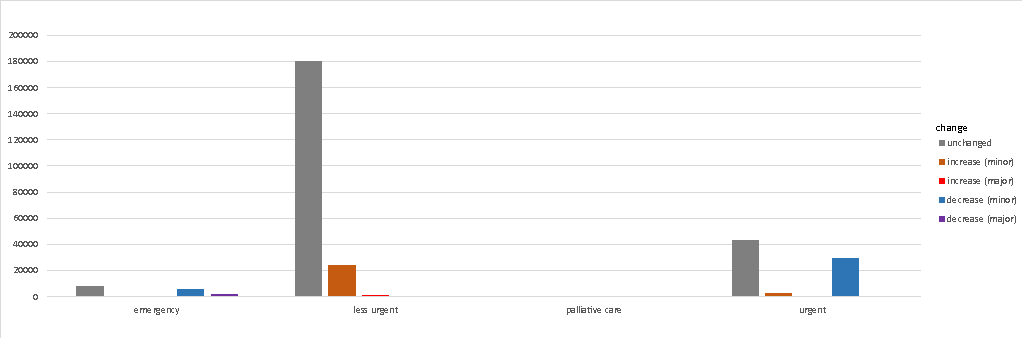
\includegraphics[page=1,width=1.8\textwidth]{graph-change.pdf}
      }
      \caption{Priority assigned to patient cases.}
      \label{fig:caller-priority}
   \end{figure*}
\end{landscape} 
 
 \begin{landscape}
   \begin{figure*}[]
   
      \centering
      \framebox{\parbox{2.5in}{
}
      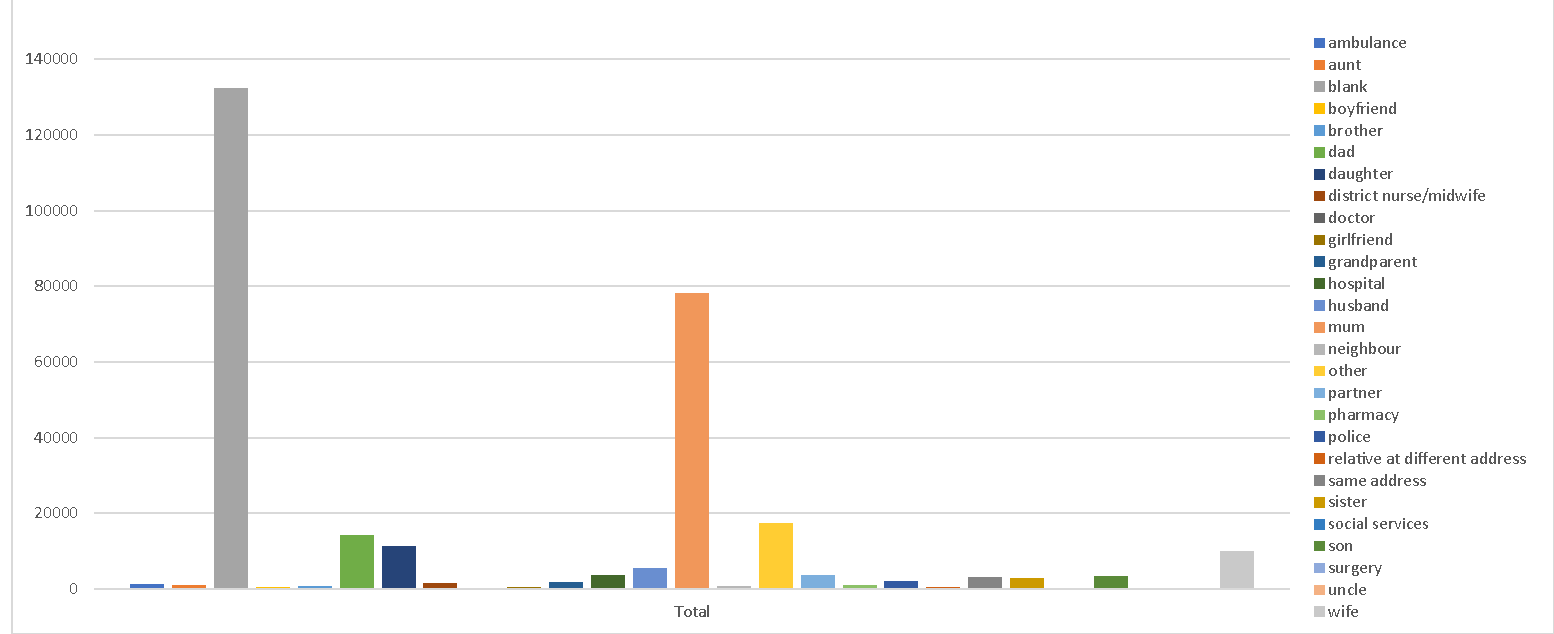
\includegraphics[page=1,width=1.8\textwidth]{graph-caller+.pdf}
      }
      \caption{EHR parameter relating to patient relationship to caller, showing
high dimensionality and large volume of null values.}
      \label{fig:caller-relationship}
   \end{figure*}
\end{landscape} 


 
 \begin{figure}[]
   \centering
   \begin{tabular}{@{}c@{\hspace{.1cm}}c@{}}
 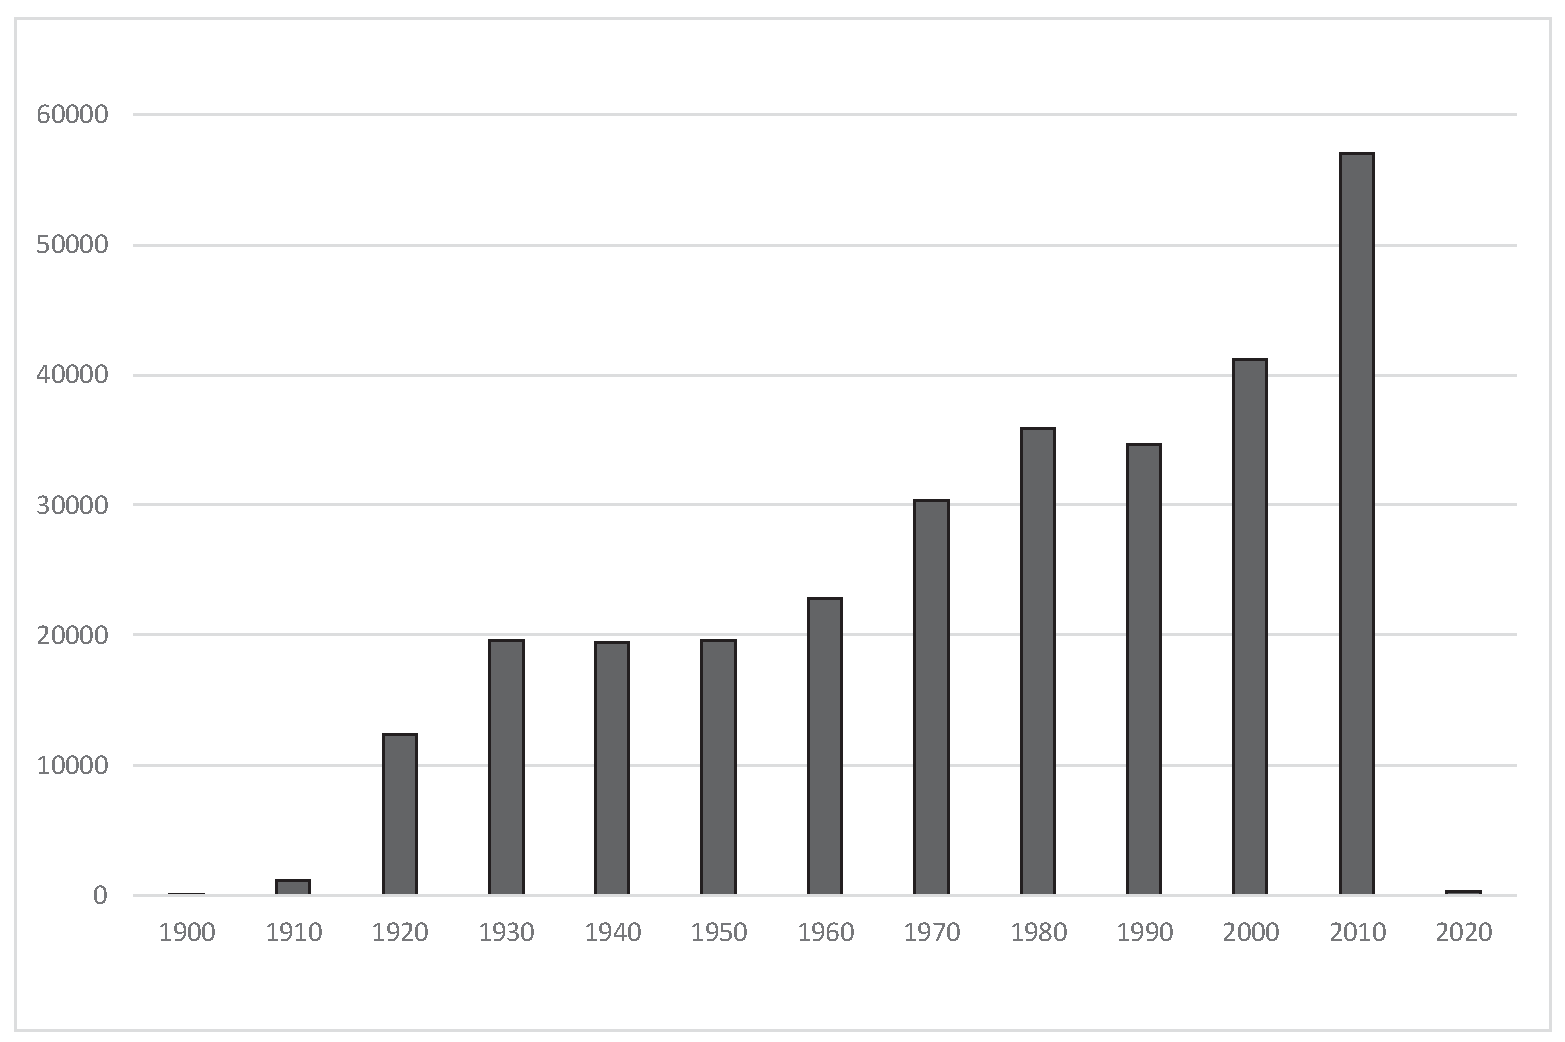
\includegraphics[page=1,width=1.00\textwidth]{dob-fas.pdf} & 
   \end{tabular}
  \caption{EHR\index{Electronic Health Record} parameter relating to patient date of birth.}
 \label{fig:caller-age}
\end{figure}

      \begin{figure}[ht]
   \centering
   \begin{tabular}{@{}c@{\hspace{.2cm}}c@{}}
 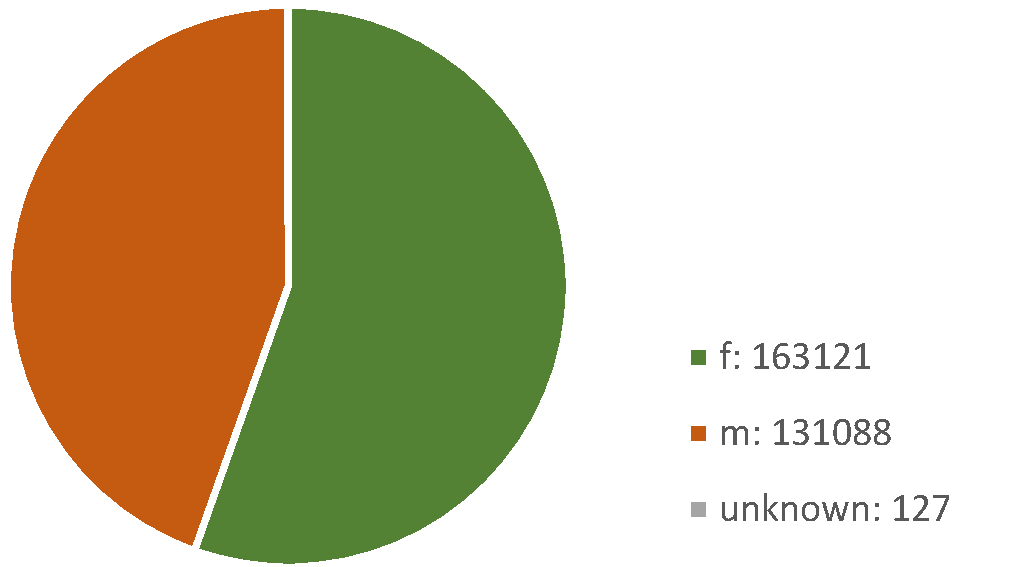
\includegraphics[page=1,width=0.60\textwidth]{graph-sex2.pdf} & 
   \end{tabular}
  \caption{Sex ratio of cases.}
 \label{fig:caller-sex}
\end{figure}




   \begin{figure}[ht]
   \centering
   \begin{tabular}{@{}c@{\hspace{.2cm}}c@{}}
 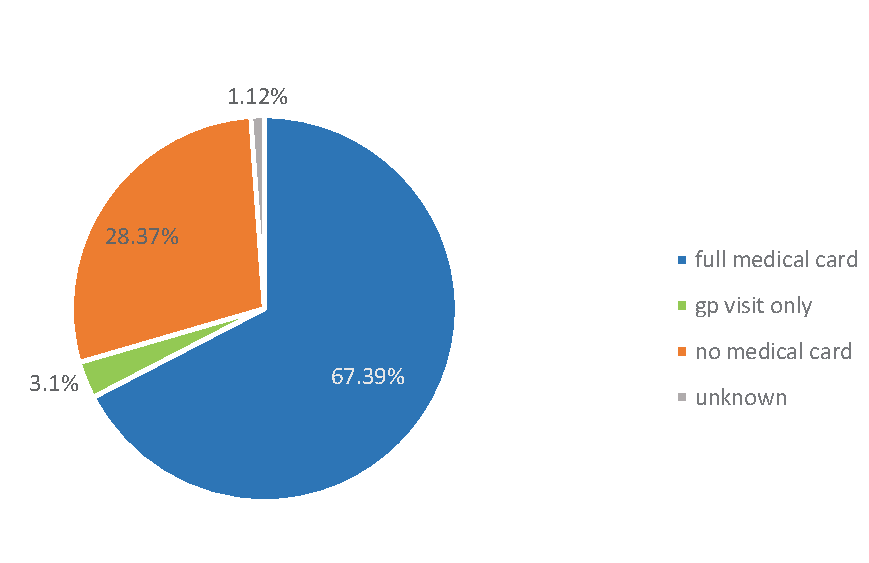
\includegraphics[page=1,width=0.80\textwidth]{Figs/graph-medical-card2.pdf} & 
   \end{tabular}
  \caption{Medical card status of patients.}
 \label{fig:caller-card}
\end{figure}
 
   There were some interesting non-numerical attributes relating to cases available within this research. This included the priority assigned to cases by call-operators (Figure \ref{fig:caller-priority}). The assigned priority could be changed (sometimes radically) after nurse triage, but typically this value wasn't altered. The vast majority of cases were classified as `less urgent'  The only other common classification was that of `urgent', but almost  half of these cases were downgraded to `less urgent' after assessment. The description of `less urgent ', and even to a lesser extent, ` urgent' are both very broad, and their consequent vagueness undercuts their capacity to provide insight into cases. For instance, these descriptions provide no indicator whether the cases in question relate to chronic or acute conditions. It is also unclear what precipitated the change of status of some of these cases from their initial handling by call centre staff, to nurse triage. 
%    \begin{figure}[h]
%   \centering
%   \begin{tabular}{@{}c@{\hspace{.2cm}}c@{}}
% 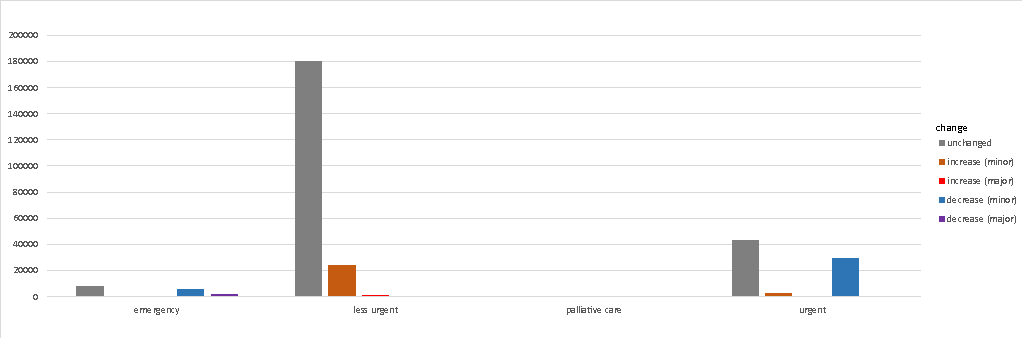
\includegraphics[page=1,width=1.20\textwidth]{graph-change.pdf} & 
%   \end{tabular}
%  \caption{Priority assigned to patient cases.}
% \label{fig:caller-priority}
%\end{figure}
 
 
 
 
% \begin{figure}[]
%   \centering
%   \begin{tabular}{@{}c@{\hspace{.2cm}}c@{}}
% 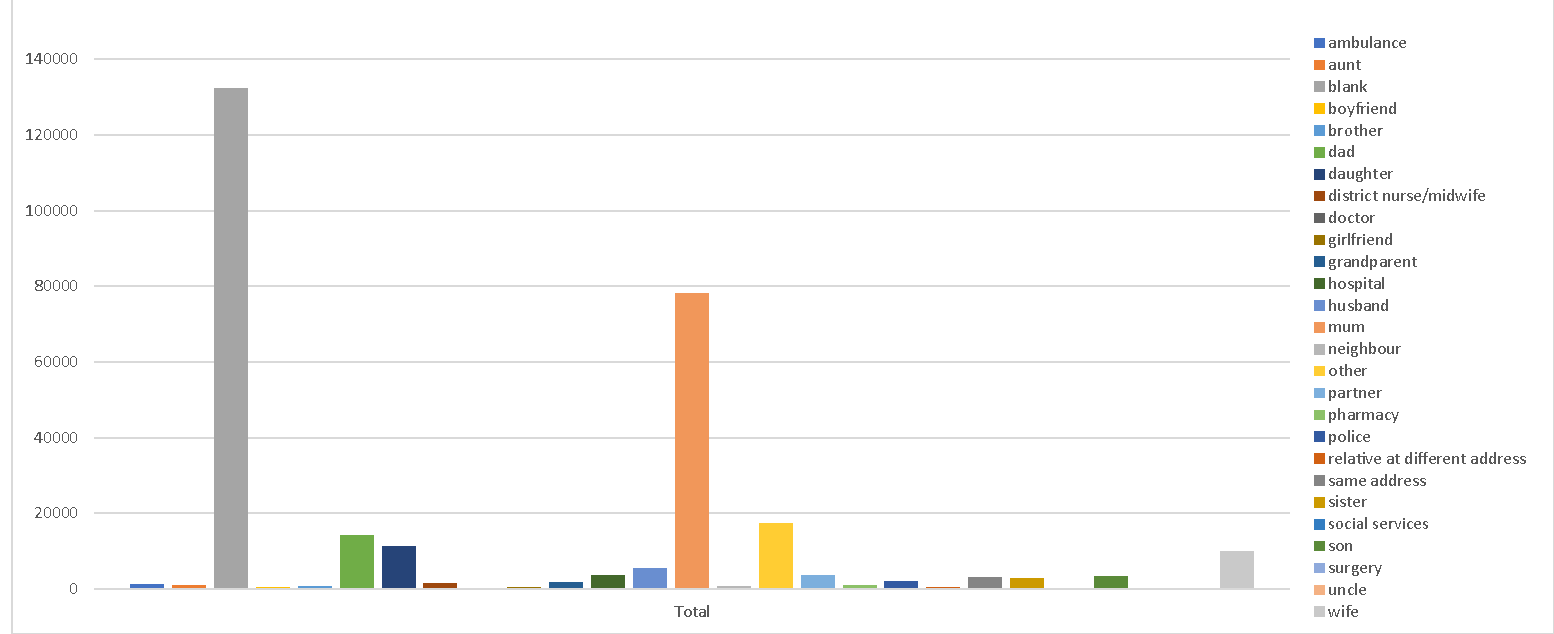
\includegraphics[page=1,width=1.20\textwidth]{graph-caller+.pdf} & 
%   \end{tabular}
%  \caption{EHR\index{Electronic Health Record} parameter relating to patient relationship to caller, showing high dimensionality and large volume of null values.}
% \label{fig:caller-relationship}
%\end{figure}
 
 

 
 Another interesting feature is that which describes the patient's `relationship to caller' - that is to say, the patient's relationship to the person who has actually called Caredoc\index{Caredoc}. Unfortunately this attribute was mostly filled with nulls. Where a value was recorded, the term `mum' was disproportionately represented. Values were otherwise sparse, as can be seen in Figure \ref{fig:caller-relationship}. It is difficult to determine, after the fact, whether this attribute was reliably populated by Caredoc\index{Caredoc} staff. For instance, it is not known whether a lack of information relating to this attribute consistently means that the patient themselves was the caller.
 

 
 Date of patient birth (binned by decade) can be seen in Figure \ref{fig:caller-age}. The small number of cases with no \hl{recorded date of birth (demarcated by `2020') is visible here (though it is possible that patients with a date of birth recorded as `1900' are also erroneous). While there a a large number of very young children (under the age of 4) treated as part of the total volume of cases, these still account for only 19\% of the total.}   
 

 
As may be apparent, demographic data was very limited, with most parameterised information being metadata relating to the call itself. The only demographic data recorded by Caredoc\index{Caredoc} related to the age, sex, medical card status, and address of the patients (the latter of which was not provided by Caredoc\index{Caredoc} in data related to this research). Parametric information detailing the sex of the patient can be seen in Figure \ref{fig:caller-sex}, and detailing the medical card status can be seen in Figure \ref{fig:caller-card}.  These features both had a small set of values, with little  noise.  
 

 
 Initial attempts to classify patients as either frequent or non-frequent users was performed using \hl{ the attributes discussed above} using Random Forest, linear SVM, and multivariate linear regression, as can be seen in Chapter \ref{chpt:machine-learning}.  
 

 
 
 
 \subsection{Free-text data}
 \label{section:free-text-description}
 
 \begin{table}[ht]
\setlength{\tabcolsep}{8pt}
   \ra{1.2}

\centering
\caption{Free-text data in corpus.}
\label{table:corpus}
\begin{tabular}{@{}lcccc@{}}
\toprule
\textbf{attribute} & \textbf{entries} & $\mathbf{\bar{c}}$ & $\mathbf{\bar{w}}$ &$\mathbf{\sigma w}$ \\ \midrule
olc\_history       & 15226            & 182.72                       & 16.58 & 23.4                      \\
olc\_examination   & 11326            & 115                          & 7.24  &11.9                      \\
olc\_diagnosis     & 120433           & 25.46                        & 1.66  & 3.65                      \\
olc\_treatment     & 123517           & 74.86                        & 5.61      &9.38                  \\
teleguides         & 58906            & 271.28                       & 38.95     &20.05                     \\ \bottomrule
\end{tabular}
\end{table}
 
 The vast majority of information relating to cases was recorded in the free text fields (of which there were four attributes, as can be seen in Table \ref{table:corpus}, where average count of word (w) and characters (c) is described, along with the standard deviation of word count $\mathbf{\sigma}w$). The `olc\_' delineation is a naming convention within Caredoc's relational database management system which indicates the presence of FTN.\index{free-text} The `teleguides' field has a slightly different use case, where it relates to free text notes concerning the use of the Nightingale system (described in Section \ref{Out-Of-Hours_Health-Care}). teleguides notes did not coexist with notes relating to any of the other four FTN fields. 
 These fields (the names of which in Table \ref{table:corpus} are taken directly from the Caredoc databases) were not consistently filled for each case treated, and the actual population of these separate fields only loosely corresponded to their purported purposes (of history, examination, diagnosis, or treatment of patients respectively). When more than one of these fields was filled, their usage was however consistently recorded in this temporal order. Consequently, if simultaneously present for a given case, these data were appended together when creating datasets for our classifiers.
 
 \newcommand*{\thead}[1]{\multicolumn{1}{c}{\bfseries #1}}
\begin{comment}
\begin{table}[h]
   \ra{1.3}
\caption{Free-text data in corpus}
\begin{center}
\begin{tabular}{|l|l|l|l|}
\hline
\textbf{attribute}     & \textbf{entries} & $\mathbf{\vert\bar{c}\vert}$ & $\mathbf{\vert\bar{w}\vert}$   \\
\hline
olc\_history   & 15226  & 182.72 & 16.58 \\

olc\_examination & 11326  & 115 & 7.24 \\

olc\_diagnosis & 120433  & 25.46  & 1.66  \\

olc\_treatment    & 123517  & 74.86  & 5.61 \\

teleguides & 58906 & 271.28 & 38.95 \\
\hline
\end{tabular}
\end{center}
\label{table:free-text}
\end{table}
\end{comment}

 % Please add the following required packages to your document preamble:
% \usepackage{booktabs}

 


 Decision support systems based upon predicative analysis have had limited application in real world environments. One of the reasons for this is that EHR\index{Electronic Health Record} data is challenging to represent and model due to its high dimensionality, noise, heterogeneity, sparseness, incompleteness, random errors, and systematic biases \cite{botsis2010secondary}. While a wide range of parametric data was contained within the data provided, early testing showed that these fields alone were insufficient to build successful models from. We thus looked to the FTN data to provide the cornerstone of predictive analysis. The following chapter will detail measures we took to improve the features of this textual data.

The untreated corpus free-text\index{free-text} featured 131841 unique lexemes, and a linguistic diversity of 0.072 where linguistic diversity, \textit{d}, is defined as the set of terms \{\textit{t}\}, over the frequency of terms |\textit{t}| in the dataset.

\begin{comment}
\begin{align}
d: \hspace*{5mm}\left \|\frac{\left\{t\right\}}{\left \| t \right \|}  \right \|
\end{align}
\end{comment}

\begin{align}
d: \hspace*{5mm}\left |\frac{\{t\}}{|  t | }  \right |
\end{align}




 \subsection{Frequent User Data Characteristics }
 
 Frequent users are an \hl{unusual}, but significant subset of patients in our dataset. The distribution of cases relative to frequency of interaction can be seen in Figure \ref{fig:graph:cases}, showing that the vast majority of interactions with the OOHC\index{Out-of-hours Health Care} are ``non-frequent". 
 
 A balance in relation to clinical application was a significant priority; where a threshold should be adopted that would clearly establish a given patient as meriting investigation, but would not apply unnecessarily restrictive parameters on the definition of the cohort.  While the definition of frequent user based upon some temporal category was considered, this was dismissed due to a number of considerations. First, as the dataset was exclusively collected over the period of a single calendar year, there was already an implicit temporal demarcation. Second, the main concern relating to frequent users was that of persistent, unresolved medical issues, which unusually high contact over a short period of time (for instance, over the period of a couple of weeks) would not represent.
 
A working figure of 40 cases was initially established in the research as the threshold that patients were determined to be frequent users. This was later revised down to 24 cases in order to capture a larger cohort. 
 
 
A final potential means of defining frequent users lay in the absolute amount of time that patients interacted with Caredoc. This approach would deviate significantly from the way in which frequent users are typically defined \cite{holmstrom2017frequent}, but could in theory be used by specifying a certain percentile for summed consultation times over all cases for each patient. For our purposes, the mixed nature of data (relating to calls, treatment centres, and home visits), the potential for incorrect or missing data relating to the calculated duration of cases, and the fact that a threshold based upon time would be an inferior metric (compared to cases as a means of determining the frequency of interaction between patients and the OOHC in question), all told against consultation time as a means of defining a threshold.  
 
 

 
 
 Ultimately a third category of high frequent user, similar to that pursued by Bhroin et al.\cite{bhroin2019profiling}  was used to describe patients with more than what was roughly twice the baseline rate. This threshold was left at the discretion of Caredoc for potential future application on their part, as the threshold figure could easily be revised either up or down, as demanded by the organisation.  
 
 For this thesis, unless otherwise stated, frequent users will be defined as patients who had at least 24 interactions with the OOHC\index{Out-of-hours Health Care} for the calendar year of 2014. 
 
 
 
     \begin{figure}[thpb]
      \centering

      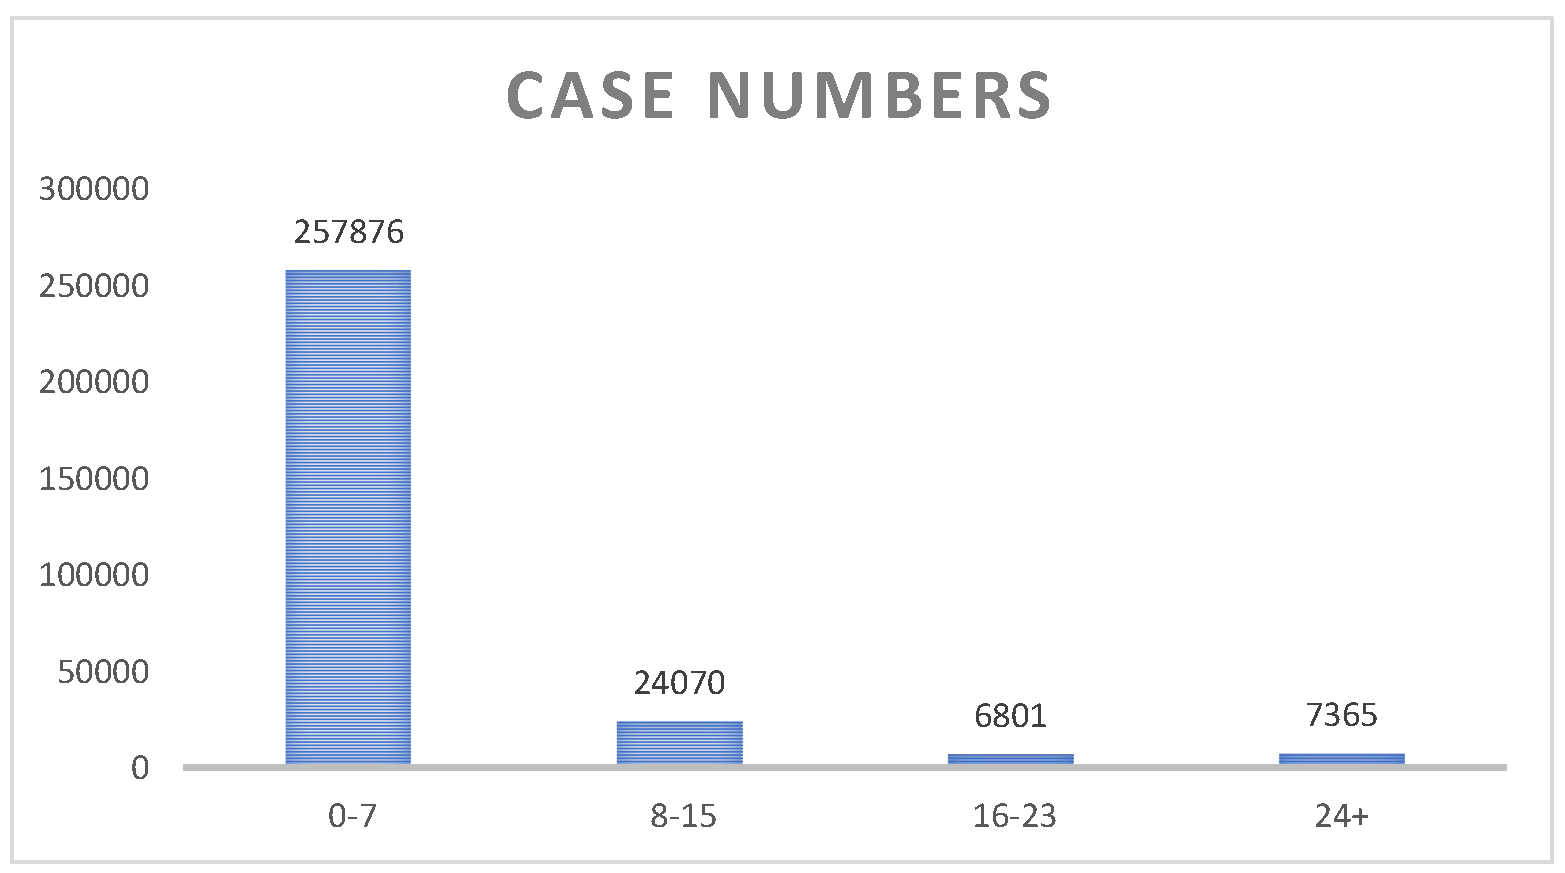
\includegraphics[scale=0.36]{graph-case-frequency.pdf}

      \caption{Case:frequency distribution}
      \label{fig:graph:cases}
   \end{figure}
   
   
As can be seen in the description of the meta data related to frequent user cases in Table \ref{table:frequent-users}, the cohort representing frequent users have a relatively similar general profile to most other users. The average age relating to frequent user cases is somewhat \hl{higher} (with a birth year mean of 1960 as opposed to 1980 for the corpus as a whole) and there's a higher prevalence of medical card holders (88\% as opposed to 67\% for the corpus as a whole). However other features do not immediately jump out as being particularly discriminative. Sex ratio and consultation times are very similar to the rest of the corpus. Priority on reception, measured from 1 (not urgent) to 4 (palliative) shows that, like the rest of the corpus, most cases belonging to this cohort were classified as `non-urgent'. \hl{Though the consultation time taken is on average slightly lower than for patients in general (7 minutes as opposed to 8 minutes), it is not statistically significant. Indeed the difference in the mean is an order of magnitude smaller than the standard deviation in this regard.}       
   
   
   
% Please add the following required packages to your document preamble:
% \usepackage{booktabs}
\begin{comment}
\begin{table}[h]
\begin{center}
\begin{tabular}{@{}l|l|l|l|l|@{}}
\cmidrule(l){2-5}
                                        & \textbf{mean} & \textbf{std} & \textbf{min} & \textbf{max} \\ \midrule
\multicolumn{1}{|l|}{dob}           & 1960.944 & 22.362 & 1919 & 2020 \\ \midrule
\multicolumn{1}{|l|}{male}          & 0.438018 & 0.4962 & 0    & 1    \\ \midrule
\multicolumn{1}{|l|}{medical\_card} & 0.886897 & 0.3167  & 0    & 1    \\ \midrule
\multicolumn{1}{|l|}{weekday}       & 3.939715 & 2.3422 & 1    & 7    \\ \midrule
\multicolumn{1}{|l|}{hour}          & 14.87261 & 6.8705 & 0    & 23    \\ \midrule
\multicolumn{1}{|l|}{priorityonreception} &	1.352342 &	0.5878 &	1 &	4 \\ \midrule

Cons\_Time\_Taken & 7.098167 & 8.4696 & 0 & 185    \\ \bottomrule
\end{tabular}
\end{center}
\end{table}
\end{comment}

% Please add the following required packages to your document preamble:
% \usepackage{booktabs}
% Please add the following required packages to your document preamble:
% \usepackage{booktabs}
\begin{table}[h]
\setlength{\tabcolsep}{8pt}
   \ra{1.2}
\centering
\caption{Description of frequent user meta-data.}
\label{table:frequent-users}
\begin{tabular}{@{}c|cccc@{}}
\toprule
\multicolumn{1}{l|}{}        & \textbf{mean} & \textbf{stdv} & \textbf{min} & \textbf{max} \\ \midrule
\textit{dob}                 & 1960.94      & 22.36        & 1919         & 2020         \\
\textit{male}                & 0.43      & 0.49        & 0            & 1            \\
\textit{medical\_card}       & 0.88      & 0.31        & 0            & 1            \\
\textit{weekday}             & 3.94      & 2.34        & 1            & 7            \\
\textit{hour}                & 14.87      & 6.87        & 0            & 23           \\
\textit{priorityonreception} & 1.35      & 0.58        & 1            & 4            \\
\textit{Cons\_Time\_Taken}   & 7.09      & 8.47        & 0            & 185          \\ \bottomrule
\end{tabular}
\end{table}




Frequent user case FTN had a general lower linguistic diversity from the rest of the corpus (0.058 to 0.072 respectively). In Chapter \ref{chpt:machine-learning} we will examine the viability of FTN, relative to parametric data, to potentially classify these cases.  


\section{Summary}

Frequent users are a complicated subset of patients. Unlike typical disease prediction, frequent usage is not in itself a specific illness, but is rather indicative of certain morbidities that are not being resolved through available primary or secondary care. Targeting frequent users with public health initiatives appears to be a priority, but the development of means to accurately predict frequent users is a complicated problem. This largely stems from the diverse characteristics of frequent users, paucity of available data, and the quality and precision of data that is available.  

Limitations concerning information relating to patients (both frequent and non-frequent users) generally stems from the restricted nature of the dataset being examined (both institutionally and temporally). As discussed earlier in this chapter, this research must be conducted without any knowledge of patient interactions with healthcare outside of Caredoc\index{Caredoc}'s auspices, nor can it consider interactions outside of 2014. However, as demonstrated with recourse to relevant literature, there is significant evidence to show both strong correlations between high use of different levels of healthcare, and the non-transitory nature of frequent user healthcare needs.

This section detailed how we created the corpus that was used throughout this research, and overcame some of the structural shortcoming the databases in our industry partner suffered from. A general description of the data was provided in this chapter, from which it is clear that significant volumes of data exist to describe cases. Nevertheless it is not obvious \textit{a priori} which features may prove most important in the classification task. 